\section{Turno de la casa}

En el turno de la casa, esta entrara en un bucle de robar cartas hasta que: llegue a 21, supere los 21 o supere tu puntaje.

Dependiendo de lo que suceda dependera si ganas, pierdes o ocurre un empate:

Si la casa supera el puntaje de 21 o si no logra superar tu puntaje, tu ganas ganando el doble de tu apuesta (ejemplo: apuestas 5000 ganas 10000):

\begin{figure}[h]
    \raggedright
    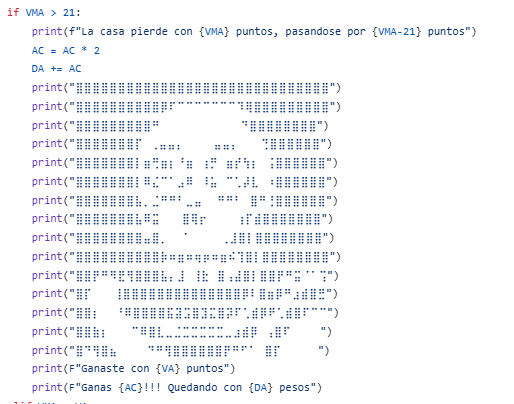
\includegraphics[width=0.4\linewidth]{Imagenes/victoria.PNG}
\end{figure}

Si la casa te supera perderás lo que apostaste:

\begin{figure}[h]
    \raggedright
    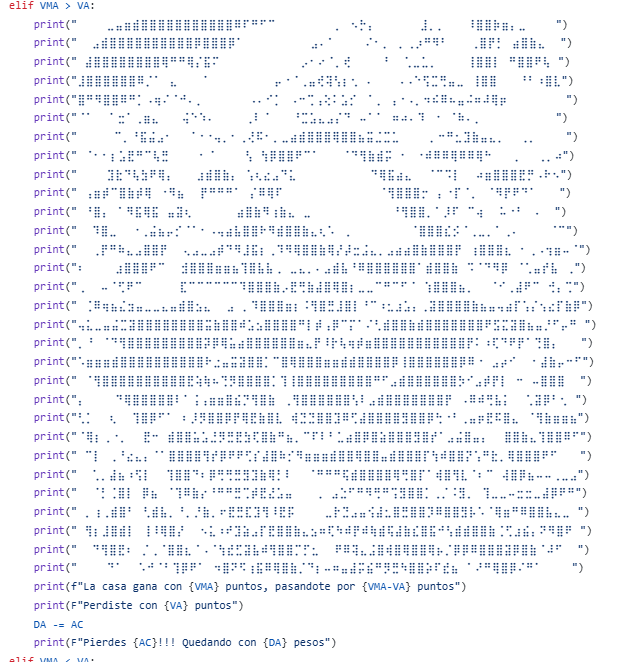
\includegraphics[width=0.3\linewidth]{Imagenes/perdida.PNG}
\end{figure}

Si la casa iguala tu puntaje sucederá un empate devolviendo te tu apuesta.

\begin{figure}[h]
    \raggedright
    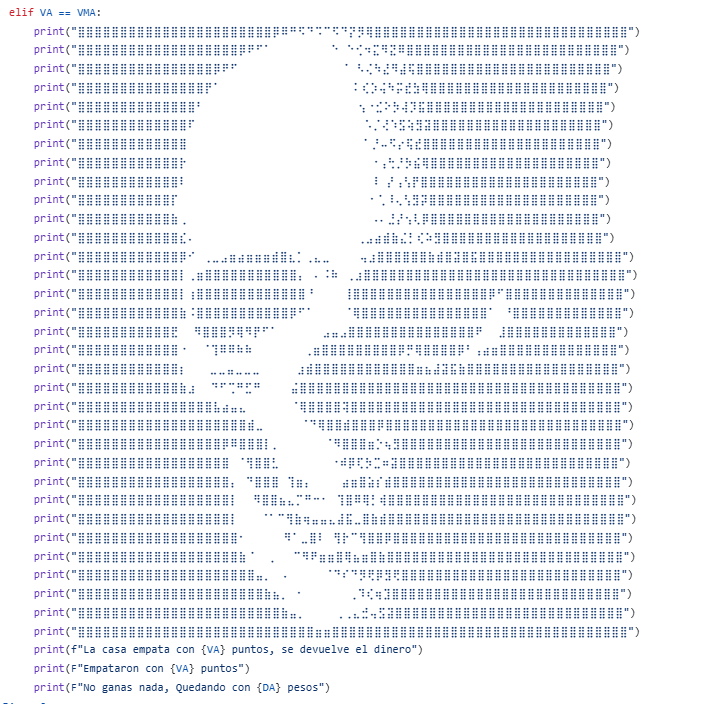
\includegraphics[width=0.3\linewidth]{Imagenes/Empate.PNG}
\end{figure}

\newpage